\documentclass[letterpaper]{article}

% AAAI header
\usepackage{aaai} 
\usepackage{times} 
\usepackage{helvet} 
\usepackage{courier}
\usepackage{url}

% fancy symbols
\usepackage{amsmath}
\usepackage{amsthm}
\usepackage{amssymb}
% \usepackage{natbib}
\usepackage{graphicx}

\newtheorem{thm}{Theorem}
\newtheorem{lemma}{Lemma}
\newtheorem{definition}{Definition}
\newtheorem{question}{Question}

\title{Classifying reviews}
\author{Ertan Dogrultan \and Cesar Romero \and Paul Wais\\
Computer Science Department \\
University of California, Los Angeles\\
Los Angeles, California 90095\\
\texttt{\{ertan,romero\}@cs.ucla.edu, pwais@ucla.edu}}

\begin{document}
\maketitle{}
\begin{abstract}
  We have an awesome translator that works for amazon and yelp reviews.
\end{abstract}

\section{Mid-quarter report}
\label{sec:mid-quarter-report}

In the report we cited~\cite{citeulike:352583} among others. Figure~

\begin{figure*}[h]
  \centering
  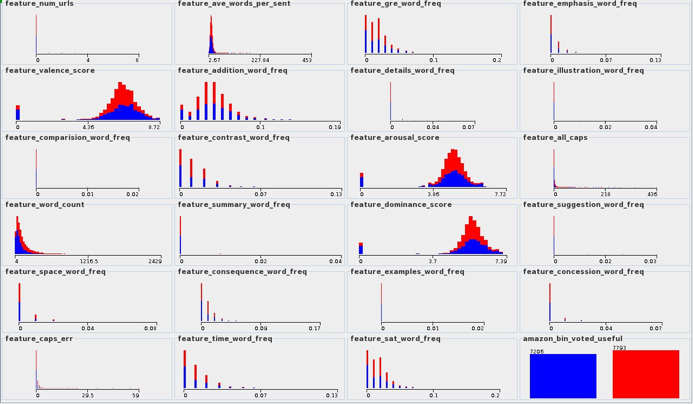
\includegraphics[scale=.5]{features_distributions}
  \caption{This is the figure from the report}
  \label{fig:dist}
\end{figure*}

\section{Features}

A concise and example-driven description of all our features.  This will probably take a little while to write :)

Link to our github:
\url{https://github.com/pwais/thumbsup}

\section{Citations to use}
Jenn's domain adaption paper \cite{JennLearnDiffDomains}\\
ANEW paper \cite{DoddsANEWPaper}\\
Pang et al sentiment classification \cite{PangSentimentClassification}\\
The WEKA paper that they ask users to cite \cite{weka} \\

\bibliography{bib}
\bibliographystyle{aaai}

\end{document}
